\documentclass[tikz,border=2pt]{standalone}
\usepackage{amsmath,amssymb}
\usepackage{tikz}
\usetikzlibrary{arrows.meta}

\begin{document}
% The OR study cycle: from the real situation through an assumed representation and a
% mathematical model to a solution, validated and implemented, with feedback loops.
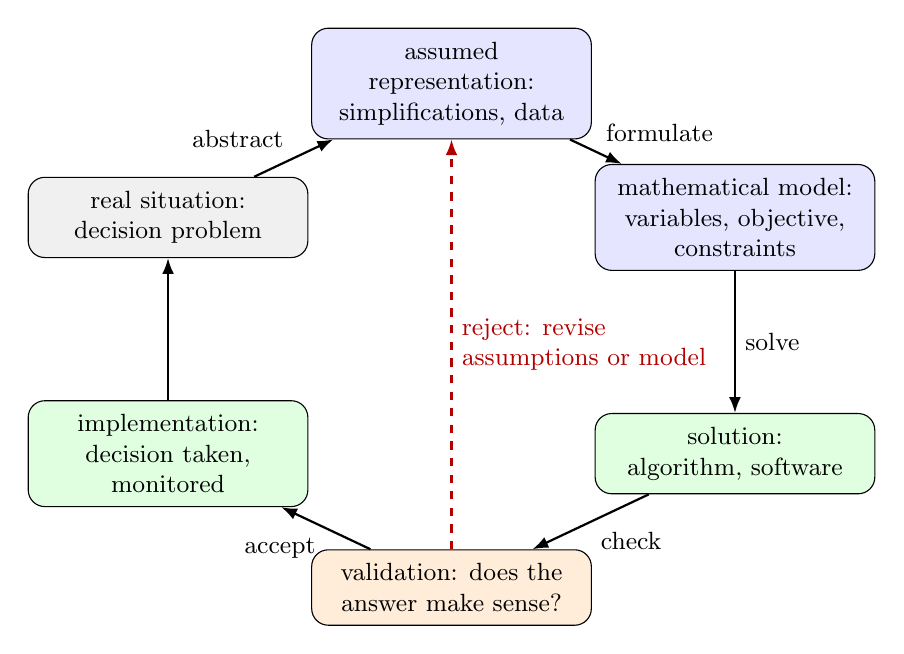
\begin{tikzpicture}[every node/.style={font=\small}, >={Latex[length=2mm]}, st/.style={draw, rounded corners=6pt, inner sep=5pt, align=flush center, text width=3.2cm, execute at begin node={\hyphenpenalty=10000\exhyphenpenalty=10000}}]
	\node[st, fill=gray!12] (a) at (0,0) {real situation:\\ decision problem};
	\node[st, fill=blue!10] (b) at (3.6,1.7) {assumed representation: simplifications, data};
	\node[st, fill=blue!10] (c) at (7.2,0) {mathematical model: variables, objective, constraints};
	\node[st, fill=green!12] (d) at (7.2,-3.0) {solution:\\ algorithm, software};
	\node[st, fill=orange!15] (e) at (3.6,-4.7) {validation: does the answer make sense?};
	\node[st, fill=green!12] (f) at (0,-3.0) {implementation: decision taken, monitored};
	\draw[->, thick] (a) -- (b) node[midway, above left] {abstract};
	\draw[->, thick] (b) -- (c) node[midway, above right] {formulate};
	\draw[->, thick] (c) -- (d) node[midway, right] {solve};
	\draw[->, thick] (d) -- (e) node[midway, below right] {check};
	\draw[->, thick] (e) -- (f) node[midway, below left] {accept};
	\draw[->, thick] (f) -- (a);
	\draw[->, thick, red!70!black, dashed] (e) -- (b) node[midway, right, align=left, red!70!black] {reject: revise\\ assumptions or model};
	\end{tikzpicture}
\end{document}
